\selectlanguage{german}
\clearpage

\section{Implementierung}

\subsection{YOLOv5}
\nameref{subsec:yolo}, ein Bilderkennungsmodell, wurde von Joseph Redmon und Ali Farhadi an der Universität von Washington entwickelt und im Jahr 2015 veröffentlicht. \nameref{subsec:yolo} steht für "You Only Look Once", was darauf hinweist, dass das Modell nur einmal auf ein Bild schaut, um Objekte schnell und präzise zu erkennen. Seit seiner Veröffentlichung wurden insgesamt neun Versionen von \nameref{subsec:yolo} veröffentlicht \cite{Yolo} .

\subsection{Das Modell}
Ein vortrainiertes Modell der fünften Version von \nameref{subsec:yolo} wird verwendet, welches bereits spezifisch für die gegebenen Anforderungen trainiert ist. Obwohl es sich um eine ältere Version von YOLOv5 handelt, ist die Effektivität des Modells nicht beeinträchtigt. YOLOv5 zeigt gerade bei begrenzten Hardware-Ressourcen wie dem Raspberry Pi 4 eine höhere Geschwindigkeit im Vergleich zu neueren Versionen wie YOLOv8. Vorteilhaft ist auch, dass eine kleinere Variante von \nameref{subsec:yolo}, nämlich Yolov5s, genutzt wird. Dieses Modell wurde mit Bildern aus diversen Quellen trainiert, wobei ein benutzerdefiniertes Datenset aus 374 Trainingsbildern und 111 Validierungsbildern erstellt wurde.

\subsection{Makesense.ai}
Für das Labeln der Daten kommt Makesense.ai zum Einsatz, eine Plattform, die es Nutzern erlaubt, Bilder hochzuladen und mit Annotationen wie Bounding Boxes und Klassifizierungen zu versehen. Dies dient der Vorbereitung von Datensätzen für Anwendungen in der Computer Vision \cite{noauthor_make_nodate}. Die Daten sind dabei in drei Klassen untergliedert: 'walking', 'sitting' und 'fall detected' (siehe Abbildung \ref{fig:yolo_classes}).


\begin{figure}[H]
	\centering
	\begin{minipage}[b]{0.3\textwidth}
		\centering
		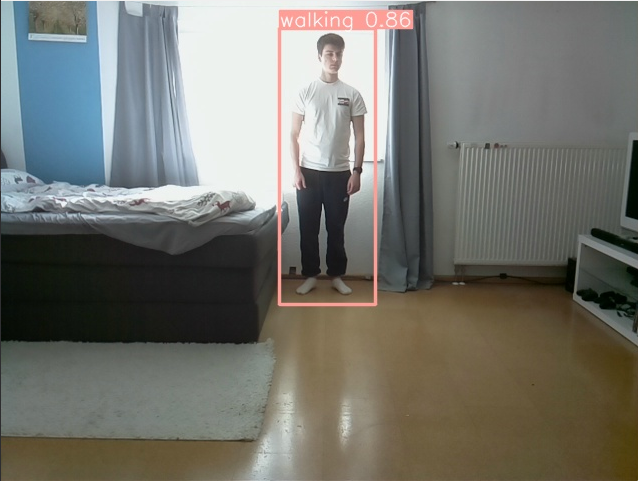
\includegraphics[width=\textwidth]{images/walking.png}
		\caption*{Klasse: ''walking''}
	\end{minipage}
	\hfill
	\begin{minipage}[b]{0.3\textwidth}
		\centering
		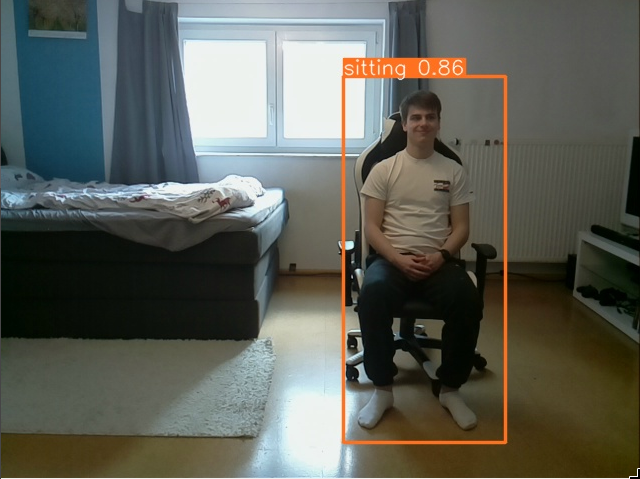
\includegraphics[width=\textwidth]{images/sitting.png}
		\caption*{Klasse: ''sitting''}
	\end{minipage}
	\hfill
	\begin{minipage}[b]{0.3\textwidth}
		\centering
		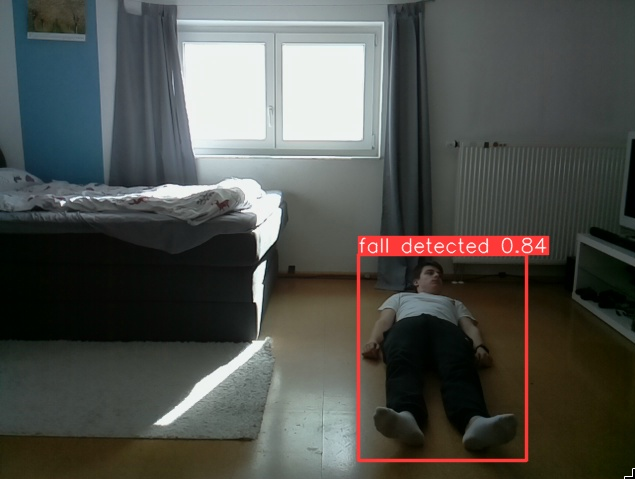
\includegraphics[width=\textwidth]{images/fallen.png}
		\caption*{Klasse: ''fall detected''}
	\end{minipage}
	\caption{YOLOv5 Detektion Klassen}
	\label{fig:yolo_classes}
\end{figure}



\subsection{Anbindung}
Die Anbindung an das YOLOv5-Modell erfolgt über PyTorch, ein Open-Source-Framework für maschinelles Lernen, das auf der Programmiersprache Python und der Torch-Bibliothek basiert. PyTorch wurde 2016 von einem Forscherteam für künstliche Intelligenz bei Facebook entwickelt \cite{noauthor_pytorch_nodate}.

Das Modell läuft in einem Docker-\nameref{subsec:container}, der kontinuierlich über MQTT einen boolean-Wert veröffentlicht, um anzuzeigen, ob ein \nameref{subsec:alarm} aufgetreten ist. Zur Einbindung der Raspberry Pi Kamera verwendet der \nameref{subsec:container} auch OpenCV, eine Open-Source-Bibliothek für Computer Vision \cite{OpenCV}. Mithilfe von OpenCV wird auch eine Funktion entwickelt, die über \nameref{subsec:mqtt} ein Bild mit allen Detektionen versendet. Diese Bilder werden später mithilfe eines weiteren \nameref{subsec:docker} Containers auf einem lokalen Rechner angezeigt.

\subsection{Evaluation}
Das Modell soll dem Model-Entwickler zufolge eine Genauigkeit von 85 bis 90\% bei Tageslicht haben. Es hat jedoch Schwierigkeiten mit der Detektion von vielen Personen auf einem Bild, was zu falschen Erkennungen führen kann. Für diesen Anwendungsfall, d.h. die Überwachung von Patienten, ist dies jedoch kein Problem, da es in den Bildern normalerweise nur einzelne Patienten gibt. 

% Zitat von wo das 85% bis 90% genauigkeit ist. Quelle fehlt, noch ergänzen.

\clearpage
\section{Matrix}

\nameref{subsec:matrix} ist einen offener Standard für interoperable, dezentrale, Echtzeitkommunikation über das Internetprotokoll (IP). Nutzer verbinden sich mit einem Heim-Server und können Räume auf jedem Matrix-Server betreten, was die Kommunikation über Servergrenzen hinweg ermöglicht. Nachrichten werden zwischen den Servern synchronisiert, was eine unterbrechungsfreie Kommunikation sicherstellt, auch wenn ein Server offline geht. \nameref{subsec:matrix} unterstützt Ende-zu-Ende-Verschlüsselung für sichere Gespräche. Zur Erprobung von \nameref{subsec:matrix} lassen sich zahlreiche Matrix-Clients verwenden \cite{noauthor_introduction_nodate}. Ein \nameref{subsec:docker} Container wird eingesetzt, um den Matrix Home-Server zu hosten \cite{noauthor_matrixdotorgsynapse_nodate}. Matrix dient dazu, Pfleger mittels eines \nameref{subsec:alarm} zu informieren.

\subsection{Element}
Der Matrix-Client Element wird für die Kommunikation genutzt \cite{noauthor_element_nodate}. Element, geleitet von den Entwicklern von \nameref{subsec:matrix}, bietet eine benutzerfreundliche Oberfläche sowie zahlreiche Funktionen, die den spezifischen Anforderungen entsprechen.

\subsection{Nginx reverse proxy}

Ein \nameref{subsec:reverseproxy} wird benötigt, damit der Matrix-Server auch \nameref{subsec:ssl} nutzen kann. Ein \nameref{subsec:reverseproxy} agiert als Vermittler zwischen Clients, wie beispielsweise Webbrowsern, und Webservern. Anstelle einer direkten Kommunikation mit dem Ursprungsserver senden Clients ihre Anfragen an den \nameref{subsec:reverseproxy}, der diese an den zuständigen Server weiterleitet und die Antworten an die Clients zurücksendet \cite{noauthor_was_nodate}. Nginx wird als \nameref{subsec:reverseproxy} verwendet \cite{noauthor_nginx_nodate}, da dieser Server umfassend dokumentiert und weit verbreitet ist. Nginx ist als \nameref{subsec:docker}-Container verfügbar, was die Integration erleichtert \cite{noauthor_nginx_nodate}.


\begin{figure}[H]
\begin{tikzpicture}[scale=0.8]
	
		\node[inner sep=0pt] (whitehead) at (-10,2)
	{
\includegraphics[width=0.15\textwidth]{images/computer.png}};
	
	\node[font=\scriptsize] at (-10,1.2) {\scriptsize Laptop 1} ;
	
	\draw[->] (-9.2,1.8)--(-6.5,0.5) node[pos=0.5, above,rotate=-28] { \scriptsize example.org};
	
		\node[inner sep=0pt] (whitehead) at (-10,0)
	{
\includegraphics[width=0.15\textwidth]{images/computer.png}};
	
		\node[font=\scriptsize] at (-10,-0.8) {\scriptsize Laptop 2};
	
		\draw[->] (-9,0)--(-6.5,0) node[pos=0.45, above] { \scriptsize example.org};
	
		\node[inner sep=0pt] (whitehead) at (-10,-2)
	{
\includegraphics[width=0.15\textwidth]{images/computer.png}};
	
			\node[font=\scriptsize] at (-10,-2.8) {\scriptsize Laptop 3};
	
		\draw[->] (-9.2,-1.8)--(-6.5,-0.5)  node[pos=0.5, above,rotate=28] { \scriptsize example.org};
	
		\node[inner sep=0pt] (whitehead) at (-5,0)
	{
\includegraphics[width=0.10\textwidth]{images/cloud.png}};
	
				\node[font=\scriptsize] at (-5,-0.8) {\scriptsize Internet};
	
		\draw[->] (-4,0)--(-1,-0);
	
	\node[inner sep=0pt] (whitehead) at (0,0)
	{
\includegraphics[width=0.10\textwidth]{images/switch.png}};
	
		\node[font=\scriptsize] at (0,-0.8) {\scriptsize reverse proxy};
	
	\draw[->] (1,0.2)--(4,0.8);
	
		\draw[->] (1,-0.2)--(4,-0.8);
	
		\node[inner sep=0pt] (whitehead) at (5,1)
	{
\includegraphics[width=0.10\textwidth]{images/switch.png}};
	
			\node[font=\scriptsize] at (5,0.4) {\scriptsize matrix server};
	
			\node[inner sep=0pt] (whitehead) at (5,-1)
	{
\includegraphics[width=0.10\textwidth]{images/switch.png}};
	
		\node[font=\scriptsize] at (5,-1.6) {\scriptsize mail server};
	
\end{tikzpicture}
	\caption{Aufbau eiens reverse proxies}
\label{fig:patient_reverse_proxy}
\end{figure}

\subsection{Postgres}
Die Einrichtung des \nameref{subsec:matrix} Docker-Containers mit PostgreSQL wird empfohlen (siehe \cite{noauthor_installation_nodate}). Standardmäßig dient SQLite als Datenbank, da es die Konfiguration vereinfacht. Für eine verbesserte Leistungsoptimierung empfiehlt es sich jedoch, PostgreSQL zu verwenden, das besser optimiert ist. PostgreSQL ist ein leistungsstarkes Datenbanksystem, das SQL verwendet und erweitert. Es bietet zahlreiche Funktionen zur sicheren Speicherung und Skalierung komplexer Datenlasten und wurde im Rahmen des POSTGRES-Projekts an der University of California in Berkeley entwickelt \cite{noauthor_postgresql_nodate}.

\subsection{Certbot}
Um die Unterstützung der \nameref{subsec:ssl}-Verschlüsselung auf dem Matrixserver sicherzustellen, ist ein \nameref{subsec:sslcertificate} notwendig. \nameref{subsec:ssl} (Secure Sockets Layer) sichert Internetverbindungen durch Verschlüsselung der Daten zwischen Browsern und Servern und gewährleistet die Vertraulichkeit sowie Integrität sensibler Informationen. Zudem ermöglicht es die Authentifizierung des Servers gegenüber dem Browser, um sicherzustellen, dass die Verbindung authentisch und sicher ist \cite{SSL}. Certbot ist ein benutzerfreundlicher Client, der ein Zertifikat von Let's Encrypt abruft.  Das \nameref{subsec:sslcertificate} von Let's Encrypt ist kostenlos. 

\subsection{Matrix Bridge}
Eine Matrix-Bridge wird verwendet, um den E-Mail-Server mit \nameref{subsec:matrix} zu verbinden \cite{jojii_jojiiofficialmatrix-emailbridge_2024}. Bridges in Matrix erleichtern die Verbindung zu anderen Plattformen und unterstützen die Interoperabilität, was die Vernetzung von Matrix über verschiedene digitale Plattformen hinweg ermöglicht \cite{noauthor_bridges_nodate}. Die Bridge gestattet es, E-Mails über Matrix zu senden und E-Mail-Inhalte in Matrix verfügbar zu machen. Alarme werden mit der Bridge, ausschließlich über E-Mail ausgelöst, die automatisch auch nach Matrix versendet wird.

